\begin{abcliste}
\abc With $r$ the distance, the nucleus with the charge $Z e$ attracts each electron with
\begin{align}
 F_\mathrm{N} &= \FKF \\
   &= \kC\times\frac{\ZO\times\left(\qe\right)^2}{\left(\re\right)^2} \\
   &= \FK \approx \result{\FKP{-9}{2}}
\end{align}

\abc
\begin{center}
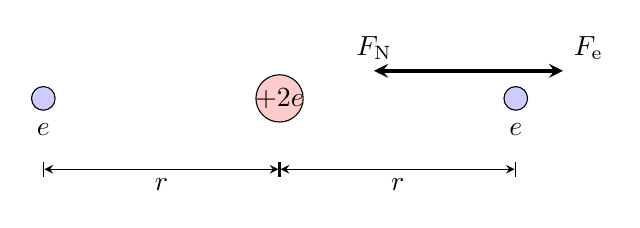
\begin{tikzpicture}[>=stealth]
 \draw[fill=blue!20] (-3,0) circle (0.15) node[below=2mm] {$e$};
 \draw[fill=red!20] (0,0) circle (0.3) node {$+2e$};
 \draw[fill=blue!20] (3,0) circle (0.15) node[below=2mm] {$e$};
 \draw[|<->|] (-3,-0.9) -- node[below] {$r$} (0,-0.9);
 \draw[|<->|] (0,-0.9) -- node[below] {$r$} (3,-0.9);
 \draw[->, very thick] (3,0.35) -- (1.2,0.35) node[above] {$F_\mathrm{N}$};
 \draw[->, very thick] (3,0.35) -- (3.6,0.35) node[above right] {$F_\mathrm{e}$};
\end{tikzpicture}
\end{center}
The other electron is $2r$ away, on the far side of the nucleus, and repels outwards:
\begin{align}
 F_\mathrm{e} &= \FeF \\
   &= \kC\times\frac{\left(\qe\right)^2}{\left(2\times\re\right)^2} \\
   &= \Fe
\end{align}
Both forces lie on one line, in opposite directions:
\begin{align}
 F &= \FF \\
   &= \FK - \Fe \\
   &= \F \approx \result{\FP{-9}{2}}
\end{align}
It points \emph{towards the nucleus}: the other electron weakens the attraction only a little.
\end{abcliste}
